
上一节的末尾,我们找出了程序在什么地方花费了大部分的执行时间。在使用“明显的”和“简单的”优化后,出现了事与愿违的情况,使程序运行速度变慢,我们也感到惊讶。现在很清楚,我们必须更详细地研究性能关键函数。

我们已经有了这样的工具:整个程序都在执行这段代码,并且有方法来测量性能。至少在我们解决了已经确定的性能问题之前是这样,我们对程序的其余部分不再感兴趣。

使用大型程序来优化几行代码有以下两个缺点:

最重要的是,尽管这几行代码是性能关键的部分,但这并不意味着程序的其余部分完全不需要时间(在我们的示例中,确实需要。但是请记住,这个示例表示正在处理的整个大型程序)。可能要等上几个小时,程序才能到达有趣的地方,要么是因为整个任务都那么长,要么是因为性能关键函数只在特定条件下调用,比如:源于网络的特定请求。

此外,处理大型程序需要更多的时间:编译和链接时间更长。实际工作可能与其他开发者所做的代码有交互,甚至编辑也需要更长时间,所以其他代码会令人分心。在这一点上,我们只对函数的基线感兴趣,所以希望能够调用这个函数,并测量结果。这就是微型基准测试的作用所在。

\subsubsubsection{2.5.1\hspace{0.2cm}微基准测试的基础概念}

简言之,微基准测试只是实现刚才描述目标的一种方式:运行一小块代码,并测量其性能。在我们的例子中,其只是一个函数,但也可能是一个更杂的代码段。重要的是,这段代码段可以在正确的初始条件下调用:对于函数,它只是参数,但对于更大的代码段,可能需要重新创建更复杂的内部状态。

我们的例子中,确切地知道需要用什么参数来调用字符串比较函数——我们构造了参数。需要做的第二件事是测量执行时间,我们已经了解了用于此目的的计时器。考虑到这一点,我们可以编写一个非常简单的基准测试,调用字符串比较函数的几个变量,并报告结果:

\begin{lstlisting}[style=styleCXX]
bool compare1(const char* s1, const char* s2) {
	int i1 = 0, i2 = 0;
	char c1, c2;
	while (1) {
		c1 = s1[i1]; c2 = s2[i2];
		if (c1 != c2) return c1 > c2;
		++i1; ++i2;
	}
}
bool compare2(const char* s1, const char* s2) {
	unsigned int i1 = 0, i2 = 0;
	char c1, c2;
	while (1) {
		c1 = s1[i1]; c2 = s2[i2];
		if (c1 != c2) return c1 > c2;
		++i1; ++i2;
	}
}
int main() {
	constexpr unsigned int N = 1 << 20;
	unique_ptr<char[]> s(new char[2*N]);
	::memset(s.get(), 'a', 2*N*sizeof(char));
	s[2*N-1] = 0;
	system_clock::time_point t0 = system_clock::now();
	compare1(s.get(), s.get() + N);
	system_clock::time_point t1 = system_clock::now();
	compare2(s.get(), s.get() + N);
	system_clock::time_point t2 = system_clock::now();
	cout << duration_cast<microseconds>(t1 - t0).count() <<
	  "us " << duration_cast<microseconds>(t2 - t1).count() <<
	  "us" << endl;
}
\end{lstlisting}

这个程序中,我们只测试两个比较函数,它们都没有循环结束条件,一个用\texttt{int}型索引,另一个用\texttt{unsigned int}型索引。另外,我们将不会在后面的代码清单中重复\texttt{\#include}和\texttt{using}语句。输入数据只是一个长字符串,从头到尾填充了相同的字符,所以子字符串的比较将一直进行到字符串的末尾。当然,可以根据需要的任何数据进行基准测试,我们先从最简单的情况开始。

这个程序看起来会做我们需要的事情:

%\hspace*{\fill} \\ %插入空行
\begin{center}
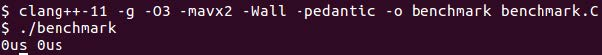
\includegraphics[width=0.9\textwidth]{content/1/chapter2/images/22.jpg}\\
图 2.22
\end{center}

不管怎样,都是0耗时。到底是哪里出错了呢?也许,单个函数调用的执行时间太快而无法测量?这是一个不错的想法,我们可以很容易地解决这个问题:如果一个调用的时间太短,只需要多调用几次:

\begin{lstlisting}[style=styleCXX]
int main() {
	constexpr unsigned int N = 1 << 20;
	constexpr int NI = 1 << 11;
	unique_ptr<char[]> s(new char[2*N]);
	::memset(s.get(), 'a', 2*N*sizeof(char));
	s[2*N-1] = 0;
	system_clock::time_point t0 = system_clock::now();
	for (int i = 0; i < NI; ++i) {
		compare1(s.get(), s.get() + N);
	}
	system_clock::time_point t1 = system_clock::now();
	for (int i = 0; i < NI; ++i) {
		compare2(s.get(), s.get() + N);
	}
	system_clock::time_point t2 = system_clock::now();
	cout << duration_cast<microseconds>(t1 - t0).count() <<
	  "us " << duration_cast<microseconds>(t2 - t1).count() <<
	  "us" << endl;
}
\end{lstlisting}

我们可以增加迭代次数\texttt{NI}直到得到结果,对吧?不可能那么快的:

%\hspace*{\fill} \\ %插入空行
\begin{center}
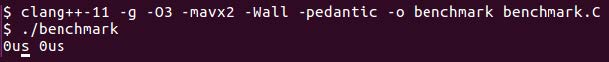
\includegraphics[width=0.9\textwidth]{content/1/chapter2/images/23.jpg}\\
图 2.23
\end{center}

确实太快了,但为什么呢?让我们在调试器中逐步检查这个程序,看看它实际上做了什么:

%\hspace*{\fill} \\ %插入空行
\begin{center}
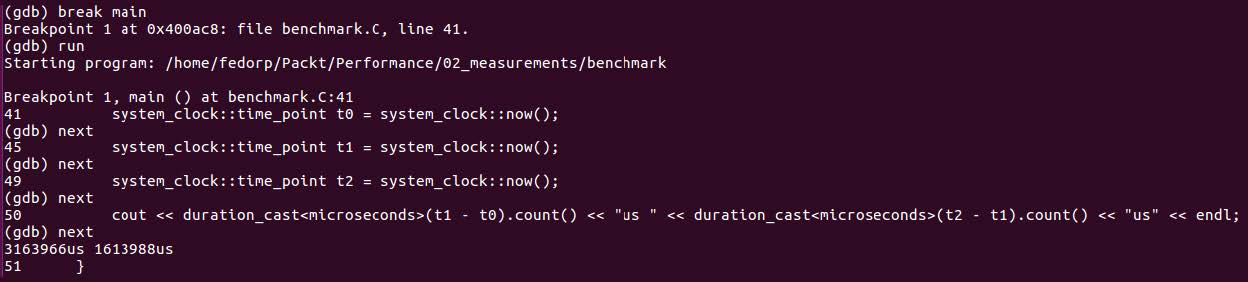
\includegraphics[width=0.9\textwidth]{content/1/chapter2/images/24.jpg}\\
图 2.24
\end{center}

我们在\texttt{main}函数中设置了断点,所以程序一启动就会暂停,然后我们一行一行地执行程序……不过,这并不是我们写的所有的代码行!剩下的代码在哪里?我们可以猜测这是编译器的原因,但是为什么呢?我们需要了解更多关于编译器优化的知识。

\subsubsubsection{2.5.2\hspace{0.2cm}微基准测试和编译器优化}

要理解神秘的缺失代码,我们必须看下这里做了什么。其创建一些字符串,调用比较函数,并且……没有了?!没有别的事情发生。除了在调试器中滚动观察代码外,如何通过运行这个程序来知道代码是否执行了呢?没有其他办法。早在我们之前,编译器就得出了同样的结论。开发者无法区分执行和不执行部分代码的区别,编译器已经对其进行了优化。但是,开发者可以分辨出区别:什么都不做比做某事花费的时间要少得多。这里,我们可以从C++标准中得到一个非常重要的概念它对理解编译器优化至关重要:可观察行为。

标准表示,编译器可以对程序进行任何更改,只要这些更改不会改变可观察对象的行为即可。标准对于什么构成了可观察行为也非常具体:

\begin{enumerate}
\item 对不稳定(volatile)对象的访问(读和写)需要严格按照发生它们的表达式的语义进行。特别是,对于同一线程上其他不稳定对象的访问,编译器不能重排。

\item 程序终止时,写入文件的数据与写入程序执行时的数据一样。

\item 发送到交互设备的提示文本,将在程序等待输入之前显示出来。简单地说,输入和输出操作不能省略或重排。
\end{enumerate}

上述规则有几个例外,但没有一个适用于我们的程序。编译器必须遵循假设规则:经过优化的程序应该显示与所写完全一样的可观察行为,一行一行地执行。请注意,因为调试器下运行程序并不构成可观察行为,所以调试器中会有代码缺失。它的执行时间很长,不执行看起来也无所谓,所以编译器为了优化程序,就略过了执行。

在新理解下,让我们再来看看基准代码:字符串比较的结果不会以任何方式影响可观察行为,因此整个计算可以由编译器自行决定。我们的观察也找到了解决这个问题的方法,必须确保计算的结果影响可观察行为。一种方法是利用前面描述的volatile语义:

\hspace*{\fill} \\ %插入空行
\noindent
\textbf{05\_compare\_timer.C}
\begin{lstlisting}[style=styleCXX]
int main() {
	constexpr unsigned int N = 1 << 20;
	constexpr int NI = 1 << 11;
	unique_ptr<char[]> s(new char[2*N]);
	::memset(s.get(), 'a', 2*N*sizeof(char));
	s[2*N-1] = 0;
	volatile bool sink;
	system_clock::time_point t0 = system_clock::now();
	for (int i = 0; i < NI; ++i) {
		sink = compare1(s.get(), s.get() + N);
	}
	system_clock::time_point t1 = system_clock::now();
	for (int i = 0; i < NI; ++i) {
		sink = compare2(s.get(), s.get() + N);
	}
	system_clock::time_point t2 = system_clock::now();
	cout << duration_cast<microseconds>(t1 - t0).count() <<
	  "us " << duration_cast<microseconds>(t2 - t1).count() <<
	  "us" << endl;
}
\end{lstlisting}

对比较函数的每次调用的结果都需要写入一个volatile变量中,并且根据标准,这些值必须正确,且以正确的顺序写入。编译器现在别无选择,只能调用比较函数并获得结果。只要结果本身不变,计算这些结果的方法仍然可以优化。这正是我们想要的:我们希望编译器为比较函数生成最好的代码,最好是在实际程序中生成的代码,但不想让它完全放弃这些功能。运行这个基准测试表明我们终于实现了我们的目标,代码肯定会运行:

%\hspace*{\fill} \\ %插入空行
\begin{center}
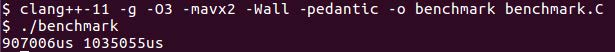
\includegraphics[width=0.9\textwidth]{content/1/chapter2/images/25.jpg}\\
图 2.25
\end{center}

第一个值是\texttt{compare1()}函数的运行时,该函数使用\texttt{int}型索引,它确实比\texttt{unsigned int}版本略快一些(暂时不要太相信这些结果)。

将我们的计算与某些可观察行为纠缠在一起的第二个选择是,将结果打印出来,这可能会有点棘手。考虑一下简单的修改:

\begin{lstlisting}[style=styleCXX]
int main() {
	constexpr unsigned int N = 1 << 20;
	constexpr int NI = 1 << 11;
	unique_ptr<char[]> s(new char[2*N]);
	::memset(s.get(), 'a', 2*N*sizeof(char));
	s[2*N-1] = 0;
	bool sink;
	system_clock::time_point t0 = system_clock::now();
	for (int i = 0; i < NI; ++i) {
		sink = compare1(s.get(), s.get() + N);
	}
	system_clock::time_point t1 = system_clock::now();
	for (int i = 0; i < NI; ++i) {
		sink = compare2(s.get(), s.get() + N);
	}
	system_clock::time_point t2 = system_clock::now();
	cout << duration_cast<microseconds>(t1 - t0).count() <<
	  "us " << duration_cast<microseconds>(t2 - t1).count() <<
	  "us" << sink << endl;
}
\end{lstlisting}

注意,变量\texttt{sink}不再是volatile类型。相反,我们输出了它的最终值。不过,这并不像想象的那样有效:

%\hspace*{\fill} \\ %插入空行
\begin{center}
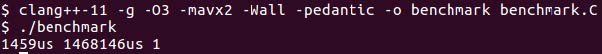
\includegraphics[width=0.9\textwidth]{content/1/chapter2/images/26.jpg}\\
图 2.26
\end{center}

函数\texttt{compare2()}的执行时间与以前大致相同,但\texttt{compare1()}快太多了。目前为止,我们已经足够了解这种“改进”是虚假的:编译器发现第二个调用覆盖了第一个调用的结果,因此不会影响可观察行为。

这就带来了一个有趣的问题:为什么编译器没有发现循环的第二次迭代与第一次的结果相同,并优化掉除了第一次以外的所有对比较函数的调用,对于每个函数都会这样么?如果优化器足够高级,那么它可以做到,然后我们将不得不做更多的工作来绕过它:通常,将函数编译为单独的编译单元就足以防止任何此类优化,尽管有些编译器能够进行整个程序的优化,所以在运行微基准测试时,可能要关闭这些特性。

请注意,我们的两个基准测试运行产生了一些不同的值,甚至对于没有优化的函数的执行时间也是如此。如果再次运行这个程序,可能会得到另一个值,也在相同的范围内,但略有不同。这还不够,我们需要的不仅仅是大概的数字。我们可以多次运行基准测试,计算需要重复多少次,并计算平均时间,但无需手工操作。不必编写代码来完成此任务,因为已经有这样的代码了,并且可以作为微基准测试工具使用。我们现在就来学习一种这样的工具。

\subsubsubsection{2.5.3\hspace{0.2cm}谷歌基准测试工具}

编写一个微型基准测试需要大量的样板代码,主要用于度量时间和累加结果。此外,该代码对测量的准确性至关重要。有几个高质量的微基准库可用。本书中,我们使用谷歌基准库,下载和安装该库的说明可以在\textbf{相关准备}部分找到。本节中,我们将描述如何使用库,并解释结果。

使用谷歌基准库,我们必须编写一个小程序来准备输入并执行我们想要基准测试的代码。这是一个基本的谷歌基准程序,用于测试字符串比较函数的性能:

\hspace*{\fill} \\ %插入空行
\noindent
\textbf{10\_compare\_mbm.C}
\begin{lstlisting}[style=styleCXX]
#include "benchmark/benchmark.h"
using std::unique_ptr;
bool compare_int(const char* s1, const char* s2) {
	char c1, c2;
	for (int i1 = 0, i2 = 0; ; ++i1, ++i2) {
		c1 = s1[i1]; c2 = s2[i2];
		if (c1 != c2) return c1 > c2;
	}
}
void BM_loop_int(benchmark::State& state) {
	const unsigned int N = state.range(0);
	unique_ptr<char[]> s(new char[2*N]);
	::memset(s.get(), 'a', 2*N*sizeof(char));
	s[2*N-1] = 0;
	const char* s1 = s.get(), *s2 = s1 + N;
	for (auto _ : state) {
		benchmark::DoNotOptimize(compare_int(s1, s2));
	}
	state.SetItemsProcessed(N*state.iterations());
}
BENCHMARK(BM_loop_int)->Arg(1<<20);
BENCHMARK_MAIN();
\end{lstlisting}

每个谷歌基准测试程序都必须包括库的头文件\texttt{benchmark/benchmark.h},还要包括编译我们想要测量的代码所需的任何其他头文件(它们在前面的代码清单中)。程序本身由许多基准测试“固件”组成,每一个都只是一个具有特定签名的函数:它接受一个引用参数\texttt{benchmark::State},无返回值。该参数是谷歌基准库提供的一个对象,可以让外部开发者与基准库进行对接。

对于每个代码片段,我们需要一个固件,比如:我们想要进行基准测试的函数。在每个基准测试固件中,要做的第一件事是设置需要用作要运行的代码输入的数据。通常,需要重新创建这个代码的初始状态,以表示它在实际程序中的状态。在我们的例子中,输入是字符串,所以需要分配和初始化字符串。可以将字符串的大小硬编码到基准测试中,但也有一种方法可以将参数传递到基准测试固件中。固件使用参数字符串长度,作为\texttt{state.range(0)}的值。当然,也可以传递其他类型的参数,详细信息请参考谷歌基准库的文档。

基准测试的意义上,整个设置是随意的,因为不用测试准备数据所需的时间。测量执行时间的代码在基准测试循环的主体中,\texttt{for (auto \_: state){…}}。较老的例子中,可以发现这个循环会写成\texttt{while (state.KeepRunning()){…}},可以做着同样的事情,但效率略低。基准库来测试每次迭代所花费的时间,并决定要进行多少次迭代来累积足够的数据,以减少在度量一小段代码的运行时间时不可避免的随机噪声(只测试基准循环中代码的运行时间)。

当测量足够精确(或达到一定的时间限制)时,循环退出。对于循环,通常需要一些代码来清理前面初始化的数据,在我们的例子中,这个清理由\texttt{std::unique\_ptr}对象的析构函数进行。我们还可以调用\texttt{State}对象来输出基准测试报告的结果。基准库总是报告运行循环的一次迭代所花费的平均时间,但有时用其他方式表示程序的速度会更方便。我们的字符串比较,一个选项是报告代码每秒处理的字符数。我们可以通过调用\texttt{state}来实现。\texttt{SetItemsProcessed()}包含整个运行期间处理的字符数,每次迭代\texttt{N}个字符(或者如果想要同时计算两个子字符串,则为\texttt{2*N};项目可以计算已定义为处理单元的任何内容)。

不会因为定义了一个基准固件而发生任何事情,我们需要将它注册到库中。这里使用\texttt{BENCHMARK}宏完成,宏的参数是函数名。顺便说一下,这个名字没有什么特别,它可以是任何C++标识符;我们的以\texttt{BM\_}开头,只是遵循本书的命名惯例。\texttt{BENCHMARK}宏也是指定要传递给基准测试固件参数的地方,参数和其他基准的选项使用重载的箭头操作符传递:

\begin{lstlisting}[style=styleCXX]
BENCHMARK(BM_loop_int)->Arg(1<<20);
\end{lstlisting}

这行代码用参数\texttt{1<<20}注册基准就固件\texttt{BM\_loop\_int},这个参数可以通过调用\texttt{state.range(0)}在固件中检索。本书中,我们将看到更多不同参数的例子,可以在库文档中找到更多这样的例子。

还会注意到,前面的代码清单中没有\texttt{main()}。不过,有另一个宏\texttt{BENCHMARK\_MAIN()},这里\texttt{main()}不由我们来写,而是由谷歌基准库提供,它负责设置基准测试环境、注册基准并执行基准。

回到我们的测量,并更仔细地观察代码:

\begin{lstlisting}[style=styleCXX]
for (auto _ : state) {
	benchmark::DoNotOptimize(compare_int(s1, s2));
}
\end{lstlisting}

\texttt{benchmark::DoNotOptimize(…)}包装器的作用类似于我们之前使用的\texttt{volatile}型sink:可以确保编译器不会优化掉对\texttt{compare\_int()}的调用。注意,它实际上并没有关闭任何优化,括号内的代码会进行优化,这是我们想要的。它确实是告诉编译器表达式的结果,在我们的例子中,比较函数的返回值应该认为是“使用”,不能简单地丢弃。

现在,我们已经准备好编译,并运行第一个微基准测试了:

%\hspace*{\fill} \\ %插入空行
\begin{center}
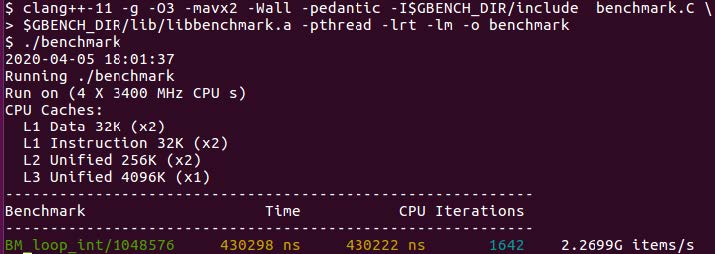
\includegraphics[width=0.9\textwidth]{content/1/chapter2/images/27.jpg}\\
图 2.27
\end{center}

编译时必须列出到谷歌基准的头文件和库路径,而谷歌基准库libbenchmark.a还依赖其他几个库。调用时,基准测试程序就会打印一些关于正在运行的系统的信息,然后执行每个已注册的固件及其参数。每个基准固件会有一行输出和一组参数,报告包括基准循环体的一次执行的平均实时时间和平均CPU时间、执行循环的次数,以及其他添加到报告中的统计信息(在我们的例子中,是通过比较每秒处理的字符数,超过2G字符/秒)。每次运行这些数据会有变化吗?如果使用正确的命令行参数启用统计信息收集,那么基准库可以为我们计算出这些数据,然后就可以进行比较了。

要重复基准测试10次并报告结果,可以这样:

%\hspace*{\fill} \\ %插入空行
\begin{center}
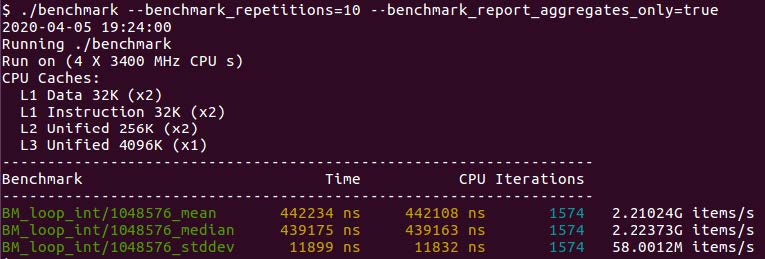
\includegraphics[width=0.9\textwidth]{content/1/chapter2/images/28.jpg}\\
图 2.28
\end{center}

看来测量结果相当准确,标准差很小。我们可以相互比较子字符串比较函数的不同实现,并找出哪个是最快的。在这之前,我得告诉你一个大秘密。

\subsubsubsection{2.5.4\hspace{0.2cm}微型基准测试不说实话}

当运行越来越多的微基准测试后,会很快会发现原因。首先,结果是有意义的,做了很好的优化,一切看起来都很好。然后做一些小的改变,就会得到非常不同的结果。回去再进行检查,现在测试给出了非常不同的数字。最后,会得到两个几乎相同的测试,但结果完全相反,这是会意识到不能再信任微基准测试了。这会摧毁对微观基准的信任,而我唯一能做的就是摧毁它,以一种可控的方式,这样我们还能从废墟中抢捞出一些有用的东西。

微基准测试和其他性能指标的基本问题是,它们很大程度上依赖于上下文。随着阅读本书的其余部分,将越来越了解现代计算机的性能行为是复杂的。结果不仅取决于代码正在做什么,还取决于系统其余部分同时在做什么,取决于它之前在做什么,以及在代码到达感兴趣的点之前执行的路径。这些东西在微观基准测试中,都不会进行复制。

相反,基准有自己的上下文。基准测试库的作者并不是没有意识到这个问题,他们尽可能地去解决这个问题。谷歌基准库在每个测试上都进行了长期测试:最初的几个迭代可能具有与运行的其余部分非常不同的性能特征,因此库会忽略最初的测量值,直到结果“稳定下来”。但这也定义了一个特定的上下文,可能与实际的程序不同。在实际的程序中,对函数的每次调用只重复一次(另一方面,有时我们会在整个程序运行过程中多次使用相同的参数调用同一个函数,所以这可能是一个不同的上下文)。

运行基准测试之前,无法在每个细节上忠实地再现大型程序的真实环境,但是有些细节很重要。目前为止,上下文差异的最大来源是编译器,或是编译器对实际程序和微基准的优化。我们已经了解了编译器试图指出,微基准测试上是一个非常慢的方法,没有做任何有用的(或至少没有可观察的),然后用更快的方法来替换它。之前使用的\textit{DoNotOptimize}包装器解决了一些由编译器优化引起的问题。

例如,编译器仍然有可能发现对函数的每次调用都返回相同的结果。此外,由于函数定义与调用点在同一个文件中,编译器可以内联整个函数,并使用可以收集到的信息来优化函数。通常情况下,当从另一个编译单元调用函数时,这种优化不可用。

为了在我们的微基准测试中更准确地还原真实情况,我们可以将比较函数移动到它自己的文件中,并编译它。我们有一个文件(编译单元),只有基准测试固件:

\hspace*{\fill} \\ %插入空行
\noindent
\textbf{11\_compare\_mbm.C}
\begin{lstlisting}[style=styleCXX]
#include "benchmark/benchmark.h"
extern bool compare_int(const char* s1, const char* s2);
extern bool compare_uint(const char* s1, const char* s2);
extern bool compare_uint_l(const char* s1, const char* s2,
unsigned int l);
void BM_loop_int(benchmark::State& state) {
	const unsigned int N = state.range(0);
	unique_ptr<char[]> s(new char[2*N]);
	::memset(s.get(), 'a', 2*N*sizeof(char));
	s[2*N-1] = 0;
	const char* s1 = s.get(), *s2 = s1 + N;
	for (auto _ : state) {
		benchmark::DoNotOptimize(compare_int(s1, s2));
	}
	state.SetItemsProcessed(N*state.iterations());
}
void BM_loop_uint(benchmark::State& state) {
	… compare_uint(s1, s2) …
}
void BM_loop_uint_l(benchmark::State& state) {
	… compare_uint_l(s1, s2, 2*N) …
}
BENCHMARK(BM_loop_int)->Arg(1<<20);
BENCHMARK(BM_loop_uint)->Arg(1<<20);
BENCHMARK(BM_loop_uint_l)->Arg(1<<20);
\end{lstlisting}

可以单独编译文件,并将它们链接在一起(必须关闭所有的程序优化)。现在,我们有了一个合理的预期,即编译器不会生成子字符串比较的某个特殊简化版本,因为它计算出了基准测试中使用的参数。通过这个简单的预防措施,结果就与我们在分析整个项目时所观察到的更加一致:

%\hspace*{\fill} \\ %插入空行
\begin{center}
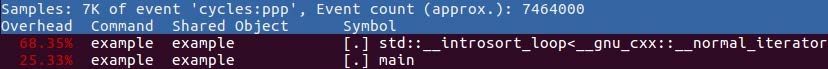
\includegraphics[width=0.9\textwidth]{content/1/chapter2/images/29.jpg}\\
图 2.29
\end{center}

代码的初始版本使用了\texttt{unsigned int}索引作为循环中的边界条件(最后一行),只要边界条件检查有完全不必要的检查就会导致惊人的性能下降(中间一行)。最后,将索引更改为\texttt{signed int}就可以恢复丢失的性能,甚至可以提高性能(第一行)。

单独编译代码片段通常足以避免不必要的优化。通常,会发现编译器会根据同一文件中的其他内容对特定的代码块进行不同的优化。这可能只是编译器中的bug,但它也可能是一些启发式的结果,根据编译器编写者的经验,这通常是正确的。你观察到结果取决于一些根本没有执行的代码,只是编译,这可能是原因。解决方案是使用实际程序中的编译单元,调用要基准测试的函数就可以了。当然,必须满足编译和链接依赖项,因此这里还需要编写模块化代码,并最小化依赖项.

其他上下文来源是计算机本身的状态。如果整个程序耗尽了内存,并在交换中循环,那么小内存的基准测试将不能代表真正的问题;另一方面,现在的问题不在“慢”代码中,问题是在其他地方消耗了太多的内存。这种上下文依赖还有更微妙的版本,并且可能会影响基准测试。这种情况的一个迹象是:结果取决于执行测试的顺序(微基准测试中,则为\texttt{BENCHMARK}宏的顺序)。重新排序测试或只运行测试的子集会得到不同的结果,它们之间存在某种依赖关系。可以是代码依赖项,通常与某些全局数据结构中的数据积累一样简单,这可能是对硬件状态的依赖。这些情况很难理解,在本书的后面,将了解一些导致这种依赖的情况。

最后,有一个上下文依赖的主要来源完全掌握在测试者手中(这未必容易避免,但至少是可以避免的),它依赖于程序的状态。我们需要处理这种依赖:要对输入进行基准测试。有时,输入是已知的或可以重构的。通常,性能问题只会发生在特定类型的输入上,我们不知道它们有什么特别之处,直到分析了这些特定输入的代码性能(这正是我们试图用微基准测试所要做的事情)。这种情况下,通常最容易从实际程序的实际运行中获取输入,并将它们存储在文件中,使用它们重新创建我们正在测试代码的状态。这个输入可以是简单的数据集合,也可以是复杂的事件序列,这些事件序列需要记录并“回放”到事件处理程序中,以重现相应的行为。

我们需要重构的状态越复杂,在部分基准测试中再现真实程序的性能行为就越困难。这个问题有点类似于编写单元测试:如果程序不能以更简单的状态分解成更小的单元,那么编写单元测试也要困难得多。这里,我们看到了设计良好的软件系统的优点:具有良好单元测试覆盖率的代码库通常更容易进行微基准测试。

正如在开始本节时所警告的那样,它的目的是在一定程度上恢复对微基准测试的信心。它们可以是一个有用的工具,正如我们将在本书中多次看到的那样,但它们也会把你引入歧途,有时甚至会走得很远。现在,请理解其中的一些原因,并更好地准备从结果中获取有用的信息,而不是完全放弃微基准测试。

我们在本章中介绍的工具没有一个能解决所有问题,它们不是万金油。而我们可以通过使用这些工具,以各种方式收集信息来达到最佳的效果,因此它们之间是相辅相成的。






